% Original fictional teaching example. Not a venue template or project result.
% Generate figure-example.pdf first; see ../README.md for the full build command.
\documentclass[10pt]{article}
\usepackage[letterpaper,margin=1in]{geometry}
\usepackage{amsmath}
\usepackage{graphicx}
\usepackage{booktabs}
\usepackage{tikz}
\usetikzlibrary{positioning,arrows.meta}
\usepackage[hidelinks]{hyperref}
\listfiles

\newcommand{\assignedrate}{\widehat{p}}
\tikzset{
  component/.style={draw,rounded corners,align=center,minimum height=10mm,
                    text width=30mm,font=\small},
  dataflow/.style={-{Stealth},thick},
}

\title{Interpretable Research Reporting: A Fictional Example}
\author{House-style demonstration}
\date{}

\begin{document}
\maketitle

\begin{abstract}
This example demonstrates a motivated metric, explicit denominators, a
regenerable figure, a restrained results table, and a semantic diagram.
All counts are fictional. They provide no evidence about this project's
agents, protocol performance, or collusion.
\end{abstract}

\section{Question and measurement}
We illustrate how to describe target-verdict rates without hiding failed trials.
The teaching question is whether treatment B has a higher observed rate than
treatment A in a hypothetical experiment. For this illustration, trials are
independently initialized with no shared memory, and success means reaching a
prespecified target verdict. Infrastructure failures count as unsuccessful
assigned trials. These assumptions must be checked for any real study.

We need a denominator that retains every assigned trial. Let $n>0$ be the number
of assigned trials and $k$ the number reaching the target verdict. Define the
assigned-trial success rate as
\begin{equation}
  \assignedrate = \frac{k}{n}.
  \label{eq:assigned-rate}
\end{equation}
Thus, a trial that fails before completion contributes to $n$, but not to $k$.
Equation~\eqref{eq:assigned-rate} estimates the declared endpoint, rather than
accuracy conditional on obtaining a verdict.

\section{Illustrative comparison and its limits}
Treatment B has an observed target-verdict rate of 45\%, compared with 30\% for
treatment A: a difference of 15 percentage points in these fictional counts.
Table~\ref{tab:counts} gives the numerators, denominators, and infrastructure
failures. Figure~\ref{fig:rates} shows marginal uncertainty under the illustrative
binomial model. These intervals alone do not test the treatment difference;
the example makes no significance or causal claim.

\begin{table}[htbp]
  \centering
  \caption{Fictional assigned-trial counts. Rates include infrastructure failures
  as unsuccessful trials; failures are also reported separately.}
  \label{tab:counts}
  \begin{tabular}{lrrrr}
    \toprule
    Treatment & Assigned & Target verdicts & Rate (\%) & Failures \\
    \midrule
    A & 40 & 12 & 30.0 & 2 \\
    B & 40 & 18 & 45.0 & 1 \\
    \bottomrule
  \end{tabular}
\end{table}

\begin{figure}[htbp]
  \centering
  % Preserve the generated 3.35-inch width; do not scale labels down.
  \includegraphics[width=3.35in]{figure-example.pdf}
  \caption{Fictional target-verdict rates. Points show 12/40 and 18/40 assigned
  trials, including 2 and 1 infrastructure failures as unsuccessful trials.
  Whiskers show 95\% Wilson score intervals assuming independent binomial trials.
  Marker shapes distinguish treatments in grayscale. No backend or model was
  run to create these teaching values.}
  \label{fig:rates}
\end{figure}

\section{An explicit system boundary}
Figure~\ref{fig:boundary} summarizes the project's actual division of authority,
as described in \texttt{docs/architecture.md}. The figure is conceptual; it
does not claim that a deployment or experiment was executed.

\begin{figure}[htbp]
  \centering
  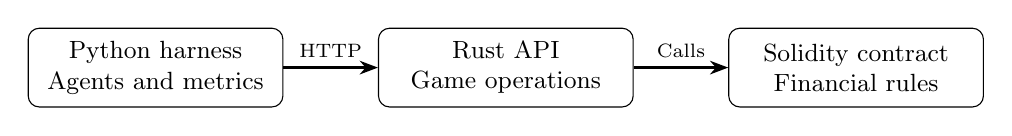
\begin{tikzpicture}[node distance=12mm]
    \node[component] (harness) {Python harness\\Agents and metrics};
    \node[component,right=of harness] (api) {Rust API\\Game operations};
    \node[component,right=of api] (contract) {Solidity contract\\Financial rules};
    \draw[dataflow] (harness) -- node[above,font=\scriptsize] {HTTP} (api);
    \draw[dataflow] (api) -- node[above,font=\scriptsize] {Calls} (contract);
  \end{tikzpicture}
  \caption{Conceptual request path from harness to contract. Arrows indicate
  submitted operations, not transfer of financial authority: settlement rules
  remain in the contract. Diagram styles are defined once in the preamble.}
  \label{fig:boundary}
\end{figure}

\section{What a real report still needs}
Replace the teaching counts with admitted run artifacts and a documented
analysis. State the actual sampling unit, dependence, comparison method,
backend, model, treatment, exclusions, and limits. Fill the paper brief and
venue record, then compile and inspect every final page using the review guide.

\end{document}
